\section{Introduction}

Social media memes can be defined as ``\emph{pieces of culture, typically jokes, which gain influence through online transmission}'' \cite{Davison2012}. More specifically, memes are visual templates usually associated with a textual caption. Analysing memes involves many unique challenges that differ from classical multimodal tasks such as image captioning and visual question answering.
While unimodal models can often perform well on multimodal datasets \citep{vqa_bias}, memes involve a lot of entanglement -- stylistic or semantic -- between the two modalities, such as the caption contradicting the image. This makes memes intrinsically multimodal.
Furthermore, pragmatics -- the context's contribution to meaning -- plays a key role in the interpretation of memes. In particular, phenomenons such as irony are challenging to detect. Even human annotators have difficulties in interpreting a meme correctly without knowledge of the community in which the meme was shared.

In this paper, we tackle the shared task on multimodal semantic role labeling of the \textsc{constraint}'22 workshop \citep{sharma2022report}.
Given a \((\text{meme}, \text{entity})\) pair,\footnote{We take each \((\text{meme}, \text{entity})\) pair as independent samples, thus considering all entities of a meme independently during training and inference.} the goal is to classify the entity's role in the meme into one of four classes (\texttt{hero}, \texttt{villain}, \texttt{victim} or \texttt{other}) from the perspective of the author of the meme.
The multimodality of the problem stems from the meme, which is given as an \((\text{image}, \text{OCR})\) pair, where OCR (for Optical Character Recognition) is the caption extracted from the image.
The dataset covers one language, English, and two domains, \textsc{covid}-19 and US politics. Figure~\ref{fig:meme} shows a sample from the training set.

Understanding memes involves a lot of commonsense and cultural knowledge on the political stance of the entities.
Thus, it requires models pre-trained on a large amount of data, capable of recognising key entities such as political figures in both modalities, and of inferring their relationship, their role and the public opinion of a community on them.
To evaluate the task's difficulty, we manually annotate a set of samples. With 5 annotators, we reach an average Macro-\fone{} of 0.65 (see details in Appendix \ref{sec:annotations}), less than 10 points above the best system submitted to the shared task.

We propose systems relying on several multimodal (vision--language) pre-trained models: One For All (OFA, \citealp{ofa}), CLIP \cite{radford2021learning} and VisualBERT \cite{li2019visualbert}.
We use these models as encoders to extract multimodal meme representations.
These \emph{encoders} are introduced in Section~\ref{sec:encoding}.
We then design several neural network classifiers to handle these representations in a task-specific fashion.
These \emph{classifiers} are presented in Section~\ref{sec:classification}.

The \textsc{constraint}'22 dataset is characterised by a large class imbalance, with the most frequent class gathering 78\% of the samples in the train set, while the least frequent one is conveyed by less than 3\% of the samples.
However, the challenge is evaluated using a Macro-\fone{} metric and calls for balanced performances across all classes.
To handle this discrepancy, we developed several subsampling strategies that we present in Section~\ref{sec:subsampling}.

Our best results are obtained by ensembling predictions from all of our models, using various ensembling methods.
The details of the ensembling methods are given in Section~\ref{sec:ensembling}.
Finally, we present our performance in Section~\ref{sec:results} along with a qualitative analysis of our models.
We highlight the limitations of the dataset, task and methods in Section \ref{sec:discussion}.

To summarise, our whole architecture is built on freely available pre-trained models.
We only fine-tune these models for the multimodal semantic role labeling task.
This makes computational training cost particularly low.
Our system can be characterised by:
\begin{itemize}[nosep]
	\item Simple classifier design on top of deep pre-trained model.
	\item Handling of class imbalance through carefully-designed sampling strategies.
\end{itemize}
Our code is available at: \url{https://github.com/smontariol/mmsrl_constraint}.

\begin{figure}[t]
    \centering
    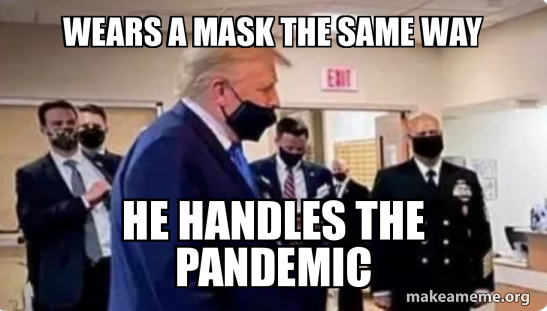
\includegraphics[width=0.8\linewidth]{figures/covid_memes_63.png}
    \caption{In this meme, the OCR is: ``WEARS A MASK THE SAME WAY\textbackslash nEXIT\textbackslash nHE HANDLES THE\textbackslash nPANDEMIC
    \textbackslash nmakeameme.org\textbackslash n''. There are two entities, ``Donald trump'' labeled as \texttt{villain} and ``mask'' labeled as \texttt{other}.}
    \label{fig:meme}
\end{figure}

